\documentclass{vldb}

\usepackage{latexsym}
\usepackage{amsmath}
\usepackage{algorithmic}
\usepackage{algorithm}
\usepackage{clrscode}
%\usepackage{epsfig}
%\usepackage{epic}
%\usepackage{eepic}
%\usepackage{xspace}
\usepackage{pst-tree}

%\addtolength{\textwidth}{1in}
%\addtolength{\oddsidemargin}{-0.5in}
%\addtolength{\evensidemargin}{-0.5in}
%\addtolength{\textheight}{0.8in}
%\addtolength{\topmargin}{-0.5in}
%\leftmargini 2.9ex


\def\punto{$\hspace*{\fill}\Box$}
\newcommand{\nop}[1]{}
\newcommand{\tuple}[1]{{\langle#1\rangle}}
\def\lBrack{\lbrack\!\lbrack}
\def\rBrack{\rbrack\!\rbrack}
\newcommand{\Bracks}[1]{\lBrack#1\rBrack}


\newtheorem{theorem}{Theorem}[section]
\newtheorem{metatheorem}{Metatheorem}[section]
\newtheorem{example}[theorem]{Example}
%\newtheorem{algorithm}[theorem]{Algorithm}
\newtheorem{definition}[theorem]{Definition}
\newtheorem{proposition}[theorem]{Proposition}
\newtheorem{property}[theorem]{Property}
\newtheorem{corollary}[theorem]{Corollary}
\newtheorem{lemma}[theorem]{Lemma}
\newtheorem{remark}[theorem]{Remark}
\newtheorem{conjecture}[theorem]{Conjecture}
\newtheorem{proviso}[theorem]{Proviso}
\newtheorem{todo}[theorem]{ToDo}

\newcommand{\comment}[1]{}
\newcommand{\compiler}{DBToaster}

\title{\compiler: A SQL Compiler for High-Performance Delta Processing in
Main-Memory Databases}
\author{Yanif Ahmad and Christoph Koch \\
Department of Computer Science \\ Cornell University, Ithaca, NY \\
\{yanif, koch\}@cs.cornell.edu}
\date{}


\begin{document}


\maketitle

\begin{abstract}
We present \compiler, a novel query compilation framework for producing high
performance compiled query executors that operate in main-memory, and
incrementally and continuously answer aggregation queries using in-memory views.
\compiler\ targets applications that require highly efficient processing of fixed
queries in the face of large input data volumes, compiling delta processing
techniques for view maintenance into simple straight-line C++ functions for
processing individual tuples. These tuple-processing functions can be highly
optimized by a C++ compiler, eliminating significant overheads involved in
interpreting query plans kept in dynamic data structures. Our compilation process
models and implements group-by aggregates as an associative map data structure,
and obtains procedures to update these maps by applying a set of map expression
rewrites, which can then easily be turned into C++ code. In this demonstration,
we show both our compilation strategy, and the significant performance
improvements our compiled executors achieve over other forms of query processing.
We are able to demonstrate orders of magnitude improvements in processing times
compared to PostgreSQL for a financial application and a data warehouse loading
application, and a factor of 5x improvement over the Stanford STREAM processing
engine in a highway toll assessment application.
\end{abstract}


\section{Introduction}
We demonstrate \compiler, a tool for compiling SQL queries into native code,
targeting main-memory databases. \compiler\ is a novel compilation framework
which generates C++ code to incrementally and continuously answer queries using
aggregate views. Our work is motivated by applications that require the highly
efficient answering of fixed workloads of aggregation queries, such as in data
stream processing, online data warehouse loading, and in financial applications.
We question the cost of highly flexible interactive query processors in such
applications, as found in today's databases with their plan interpreters and
other runtime components. In our view, a large fraction of the world's query
workloads are fixed and embedded into database application programs. Once
hardened, queries are deployed into production environments, and re\-used
numerous times, executing non-interactively.

\compiler\ is capable of compiling relational algebra with group-by aggregates by
applying rewrite rules on these repetitive or standing queries. Our rewrites
enable us to generate straight-line code exposing tuple-based execution paths to
a C++ compiler. This provides two key advantages. First, the fixed query plan
execution path can be highly optimized by a C++ compiler, enabling us to avoid
overheads that traditionally arise when query processors interpret query plans
stored in dynamic data structures. Moreover, our new delta processing techniques
are designed specifically for compilation to native code and support aggressive
inlining that leads to surprisingly small and simple straight-line code
sequences. Our compilation strategy relies on the use of a novel map algebra to
manipulate associative map data structures that are effectively main-memory
representations of group-by aggregates. We define rewrite rules that apply on
maps, enabling them to be manipulated side-by-side with relational operators
such as selections, projections and join.

\comment{
Our query rewriting defines how to process a single tuple using a precomputed
view of the remainder query and data, representing and manipulating the query via
a map algebra. The map algebra corresponds to a main-memory version of group-by
aggregates. Maintaining such views in main-memory is extremely cheap with the
use of standard pointer-based data structures and delta processing techniques.
}

In this demonstration we will put our compiler into practice by showcasing its
usage in several performance-hungry applications that are served in limited
fashion by today's data management tools, including algorithmic order book
trading, an integrated approach to data warehouse loading and analysis, as well
as stream processing applications.
As part of this demonstration, we will show our techniques are several orders of
magnitude faster than state-of-the-art   database  and significantly outperform
stream processing engines on such workloads.  In the case of queries on limit
order  book  data  as  required for  supporting  algorithmic  equities trading,
our approach currently stands alone in its ability to support realistic  data
rates  on contemporary hardware without  resorting to very substantial computing
clusters. Indeed, the memory consumption of our main-memory techniques is
sufficiently low to support applications such as data warehouse loading.



\section{DBToaster Usage}

\compiler\ is capable of compiling a wide variety of SQL queries including those
containing selections, projections, joins, and group-by aggregates. \compiler\
takes a query workload as input, as well as the data definition statements of any
tables used in the queries to determine the contents of internal datastructures,
and produces a native binary for processing the query workload over inserts,
deletes and updates on the input tables. \compiler\ focuses on applications faced
with handling a large input volume, but does not rely on artificial restrictions
of these new inputs, unlike stream processing engines, which rely on semantic
constructs such as windows or punctuations that are tightly coupled with operator
semantics. Indeed, many stream applications, such as order book trading are
self-managing, in that the application logic and usage patterns ensures state
does not grow unbounded eliminating the need for windows. Otherwise, windows may
often be expressed as predicates. \compiler\ will compile such window semantics
just as with any other part of the query, and as we will see later, efficiently
implement windowing based on the data structures used to process the windowing
predicate.

\comment{
\begin{figure}
\begin{center}
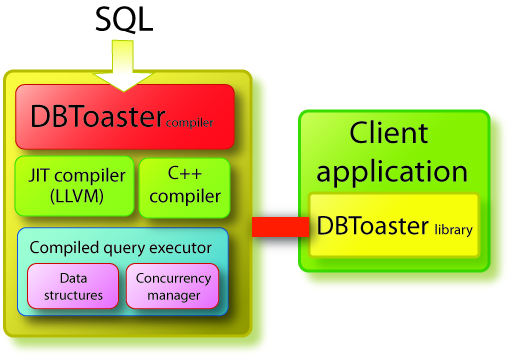
\includegraphics[scale=0.4]{figures/demo-arch}
\end{center}
\caption{\compilter\ architecture, illustrating its use as either a standalone
query processor, or as an embedded engine for direct in-memory use in client
applications.}
\label{fig:demo-arch}
\end{figure}
}

At its core, \compiler\ performs delta processing, that is each insert, delete or
update of an input table is processed through the query and produces a new
result. \compiler\ can support two types of result tuples, delta results or full
aggregate results. Internally \compiler\ computes one of these result types
depending on the type of aggregation function (for example full aggregation
results for a \texttt{max}), and maintains prior results to enable outputs of
either type. Furthermore, \compiler\ can produce both a standalone query engine
communicating both results and inputs through a socket interface, or an embedded
engine library that provides cursor-based access to full query results. This
cursor-based access is backed by internal datastructures created by \compiler\
for query processing, for example a hashtable of aggregate results keyed by
group-by columns.
\comment{
Figure~\ref{fig:demo-arch} illustrates the \compiler\ architecture.}


\section{Query Compilation}

\def\algsum{\mathrm{sum}}
\def\algagg{\mathrm{agg}}
\def\algtop{\mathrm{top}}
\def\algtopk{\mathrm{topk}}

\def\algsumr{\mbox{sumr}}
\def\algsumf{\mbox{sumf}}
\def\distinct{\mbox{distinct}}
\def\routerjoin{\bowtie\!=}

Query compilation in \compiler\ is founded on an algebra for manipulating a map
data structure. Our map algebra is related to SQL queries through the use of a
map to represent a group-by aggregate. A map algebra expression, or map for
short, is defined as one of the following forms:
\[
f_1 + f_2
\quad\;\;
f_1 * f_2
\quad\;\;
c
\quad\;\;
x
\quad\;\;
\algsumf_f(Q)
\]
where $f, f_1, f_2$ are map algebra expressions, $c$ are numerical constants,
$x$ are variables, and $Q$ are positive relational algebra
expressions.

Variables in maps are {\em free} unless they are {\em bound}. Given a map $f$
with free variables $\vec{x}$ (enumerated in the order in which they first appear
in $f$), $f[\vec{a}]$, where $\vec{a}$ is a tuple of variables and constants of
the same arity as $\vec{x}$ denotes each $x_i$ in $f$ substituted by $a_i$. The
variables $\vec{x}$ in $f[\vec{a}]$ are then called bound. So, for instance, the
free variables of $5 * x + y$ are $x,y$ and $(5 * x + y)[z, 2]$ is $5 * z + 2$
with free variable $z$. The number of free variables in a map is also called the
map's dimension.

(Positive) relational algebra expressions are built using relation names,
selection $\sigma$, projection $\pi$, relational product $\times$, union $\cup$,
constant singleton relations $\{\vec{a}\}$,
and renaming $\rho$.
Column names $A$ are treated like bound variables.
Selection conditions are comparisons
$f \;\theta\; 0$ where $\theta \in \{ =, \neq, <, \le, >, \ge \}$.
Projections may compute additional columns
using map algebra expressions, i.e.\ the syntax is
$\pi_{\vec{A}, f_1 \rightarrow B_1, \dots, f_k \rightarrow B_k}(Q)$. 

We use a multiset semantics for relations as in SQL; none of the operations
of relational algebra eliminate duplicates.
Otherwise, the semantics of relational algebra expressions $Q$ is standard.
Variables in $\vec{x}$ are {\em bound}\/ to constants from above; thus, 
the semantics of an aggregate map $\algsumf_f(Q)$ without free variables
is a single numerical value $v$ such that
\[
\algsumr_A(\pi_{f \rightarrow A}(Q))[] = \{ \tuple{v} \}.
\]
where $\algsumr$ is the ungrouped sum aggregate of SQL.

\subsection{Map compilation}
The goal of this section is to provide an algorithm for compiling map algebra
expressions into efficient C code that incrementally maintains the
maps they define.
We will need the following general-to-specific ordering $\prec$ on maps.


\begin{definition}\em
A map $f$ is called (strictly) {\em more specific than}\/ a map $f'$,
denoted $f \prec f'$, if $f$ can be obtained from $f'$ by replacing
one or more relation names occurring in $f'$ by fixed singleton relations.
\end{definition}


Note that this replacement may occur deep inside a map, not just in the topmost
relational algebra subexpression. For example,
\[
\algsumf_A(\pi_{\algsumf_B(\rho_B(\tuple{b})) + 2}(S))
\prec
\algsumf_A(\pi_{\algsumf_B(\rho_B(R)) + 2}(S))
\]


\begin{figure*}[t!]
%\begin{algorithm}
\begin{eqnarray*}
\Delta_{+R(\vec{r})} c       &:=& 0 \\
\Delta_{+R(\vec{r})} x       &:=& 0 \\
\Delta_{+R(\vec{r})} (f + g) &:=&  (\Delta_{+R(\vec{r})} f) + (\Delta_{+R(\vec{r})} g) \\
\Delta_{+R(\vec{r})} (f * g) &:=& f * (\Delta_{+R(\vec{r})} g) 
                              +   (\Delta_{+R(\vec{r})} f) * g                        
                              +   (\Delta_{+R(\vec{r})} f) * (\Delta_{+R(\vec{r})} g)
\\
\Delta_{+R(\vec{r})} \algsumf_A(\{ \vec{a} \}) &:=& 0
\\
\Delta_{+R(\vec{r})} \algsumf_{A_i}(\rho_{\vec{A}}(R)) &:=& r_i
\\
\Delta_{+R(\vec{r})} \algsumf_A(S) &:=& 0
\\
\Delta_{+R(\vec{r})}  \algsumf_A(Q_1 \cup Q_2) &:=&
\Delta_{+R(\vec{r})} (\algsumf_A(Q_1) + \algsumf_A(Q_2))
\\
\Delta_{+R(\vec{r})} \algsumf_{f[\vec{A};\dots] * g[\vec{B};\dots]}(\rho_{\vec{A}}(Q_1) \times \rho_{\vec{B}}(Q_2)) \; &:=&
\Delta_{+R(\vec{r})} \big( \algsumf_{f[\vec{A};\dots]}(\rho_{\vec{A}}(Q_1))
    * \algsumf_{f[\vec{B};\dots]}(\rho_{\vec{B}}(Q_2)) \big)
\\
\Delta_{+R(\vec{r})} \algsumf_A(\pi_{f + g \rightarrow A}(Q)) &:=&
\Delta_{+R(\vec{r})} \big( \algsumf_A(\pi_{f \rightarrow A}(Q))
   + \algsumf_A(\pi_{g \rightarrow A}(Q)) \big)
\\
\Delta_{+R(\vec{r})} \algsumf_A(\pi_{f[\vec{x}] \rightarrow A}(Q)) &:=&
   (f + \Delta_{+R(\vec{r})} f)
   * \Delta_{+R(\vec{r})} \algsumf_1(Q)
\\
\Delta_{+R(\vec{r})} \algsumf_A(\pi_{f \rightarrow A}(Q)) &:=&
   \algsumf_A(\pi_{\Delta_{+R(\vec{r})} f \rightarrow A}(Q)) \\
   &+& \algsumf_A(\pi_{f \rightarrow A}(\Delta_{+R(\vec{r})} Q)) \\
   &+& \algsumf_A(\pi_{\Delta_{+R(\vec{r})} f \rightarrow A}(\Delta_{+R(\vec{r})} Q))
\\
\Delta_{+R(\vec{r})} \algsumf_A(\sigma_{g \theta 0}(Q)) &:=&
\mbox{if ($\Delta_{+R(\vec{r})} g \;\theta\; 0$) then
   $\algsumf_A(Q + \Delta_{+R(\vec{r})}(Q))$} \\
&& \mbox{else if ($(g + \Delta_{+R(\vec{r})} g \;\theta\; 0) \Rightarrow
(g \;\theta\; 0)$) then $- \algsumf_A(Q)$ else 0}
\end{eqnarray*}
%\end{algorithm}
%
\caption{Recursive algorithm for compiling the
on insert into $R$ values $\vec{r}$ trigger.}
\label{fig:mainalg}
\end{figure*}


Figure~\ref{fig:mainalg} shows our compilation algorithm for maps, the core
procedure of the DBToaster compiler. Given a map $f$, it inductively computes a
delta-expression that does not use relational algebra.

It is easy to verify that the right-hand sides of the rewriting are successively
simpler by either being dominated by the left-hand sides under the general-to-specific
ordering $\prec$ or being sums or products of
strictly shorter expressions.

Thus, the output of the rewriting algorithm given a map is a delta map that does not
contain aggregates or relational algebra. However, the rewriting may add new free
variables, i.e., starting from a map $f[\vec{x}]$, we may obtain an aggregate-free
map $g[\vec{x}, \vec{y}]$. We then {\em marginalize}\/ over these as follows,
\[
\Delta f[\vec{x}] = \sum_{\vec{y}} g(\vec{x}, \vec{y}). 
\]

Rather than explaining the rules in full detail here, we simply note that these
rules can be thought of as being similar to pattern matching, where the right
hand side map can be used to replace any matching left hand side. Furthermore,
note that the chain of derivations directly represent the code we must generate
and execute in our tuple-processing functions.

\subsection{Compilation Example}
We briefly provide an example application of our map rewrites on the following
aggregate query:

\[
s := \algsum_{A*D}(R \bowtie S \bowtie T).
\]

For illustration we simply consider the insertion of a new tuple into
solely the relation R. Also, since this example is only meant to be a brief
illustration due to space restrictions, we omit the case for deletions.

\begin{itemize}
\item
Insert R(a,b):
\begin{eqnarray*}
\Delta s &=& \algsum_{A*D}(\{\tuple{a,b}\} \bowtie S \bowtie T)
\\ &=&
\algsum_{A*D}(\{a\} \times \sigma_{B=b}(S) \bowtie T)
\\ &=&
\algsum_{a*D}(\sigma_{B=b}(S) \bowtie T)
\\ &=&
a * \underbrace{\algsum_{D}(\sigma_{B=b}(S) \bowtie T)}_{s_D[b]}
\end{eqnarray*}

\end{itemize}

 
Next, we incrementally maintain $s_D[b]$, which in this case is maintained by
insertions into S.

\begin{itemize}
\item
Insert S(b,c):
\begin{eqnarray*}
\Delta s_D[b] &=&
\algsum_{D}(\{\tuple{b,c}\} \bowtie T)
\\ &=&
\algsum_{D}(\{b\} \times \sigma_{C=c}(T))
\\ &=&
\algsum_{D}(\sigma_{C=c}(T))
\;=:\; s_D[c]
\end{eqnarray*}
\end{itemize}

Thus the code is:
\begin{verbatim}
on insert into R values (a,b)
{
   s += a * s_D[b];

   // Updates from R to other maps...
}

on insert into S values (b,c)
{
   s += s_A[b] * s_D[c];
   s_D[b] += s_D[c];
   // Updates from S to other maps...
}

// code for T ...
\end{verbatim}



\section{Demonstration}
The \compiler\ demonstration will exhibit both the map algebra and its
transformation machinery, as well as the high performance aspect of the
project through live comparisons with alternative database implementations.
In this section we describe the application scenarios that act as motivating
use cases for \compiler, as well as the visualization tools that convey the
technical aspects of query transformations and compiled executor performance.

\subsection{Applications and workloads}
\compiler\ is suited for applications exhibiting high volumes of insertions,
deletions and updates, and in this demonstration, we show \compiler\ processing
queries for an automated trading application making use of NASDAQ TotalView order
book data~\cite{totalview-url}, TPC-H data to emulate a combined data warehouse
loading and analysis application, and finally a toll management system as
presented in the Linear Road benchmark for stream processing
engines~\cite{arasu-vldb:04}. We describe the first two applications in more
detail, referring the reader to the Linear Road paper for details on that topic.

\textbf{Processing order books in equities trading.}
Order books provide a superior view of the market microstructure for use in
trading algorithms. The bid order book consists of prices and volumes of orders
of investors who are willing to buy equities in descending price and timestamp
order, and correspondingly the ask order book indicates investors' selling
orders. Exchanges execute trades by matching the tops of the bid and ask order
books. Investors continually add, modify or withdraw limit orders, thus we view
order books as relations subject to high volumes of order inserts, updates and
deletes. Unlike stream processing scenarios \cite{motwani-cidr:03}, order
books do not grow unboundedly in practice, but cannot be expressed by windows
given their arbitrary inserts, updates and deletes. Thus in \compiler, we process
continuous queries over temporal snapshots of relations via delta processing.

We present two queries in the automated trading application, the first is a
volume-weighted average price (VWAP) query which computes the average
price-volume product of a given fraction of the total volume in the bid and
ask order book. This is used as part of the Static Order Book Imbalance (SOBI)
query which attempts to detect trade price movements indicated based on whether
there is a greater VWAP of bids than asks or vice versa. The second query is a
query to detect strategies being employed by market makes through the order
book, where market makers often submit orders to entice buyers or sellers into
the market to aid in balancing their position.

\textbf{Data warehouse loading.}
Loading large data warehouses is a computationally costly process, which
causes most data warehouse loading to be performed offline.
While commercial warehouse loaders use specialized efficient code for 
aggregation, incoming data is often the result of data integration
queries that are costly and inefficient, and with may blow up data sizes
in such a way that loading remains inefficient.
Compiling data integration and aggregation queries together yields efficient
code for loading the warehouse which may avoid the materialization of large
intermediate results.

Hence we use \compiler\ to jointly process a data integration query loading a
warehouse from OLTP databases, and an aggregation query on the warehouse. We
emulate the data integration step by using a data cleaning and transformation
query to convert a TPC-H dataset into a star schema, as described in the Star
Schema Benchmark (SSB)~\cite{poneil-ssb:07}. We then evaluate query 4.1 from SSB
on the transformed TPC-H dataset. Note this all occurs in one single query
compiled down with \compiler.

An integral part of this demonstration is to support interaction with conference
attendees, thus in addition to providing pre-cooked queries implementing these
applications, we will support compilation of a subset of SQL, namely selections,
projections, join and aggregation operations, for attendees to directly pose
their own queries on top of the base relations in these applications.




\subsection{Query compilation and code generation}

\begin{figure}
\begin{center}
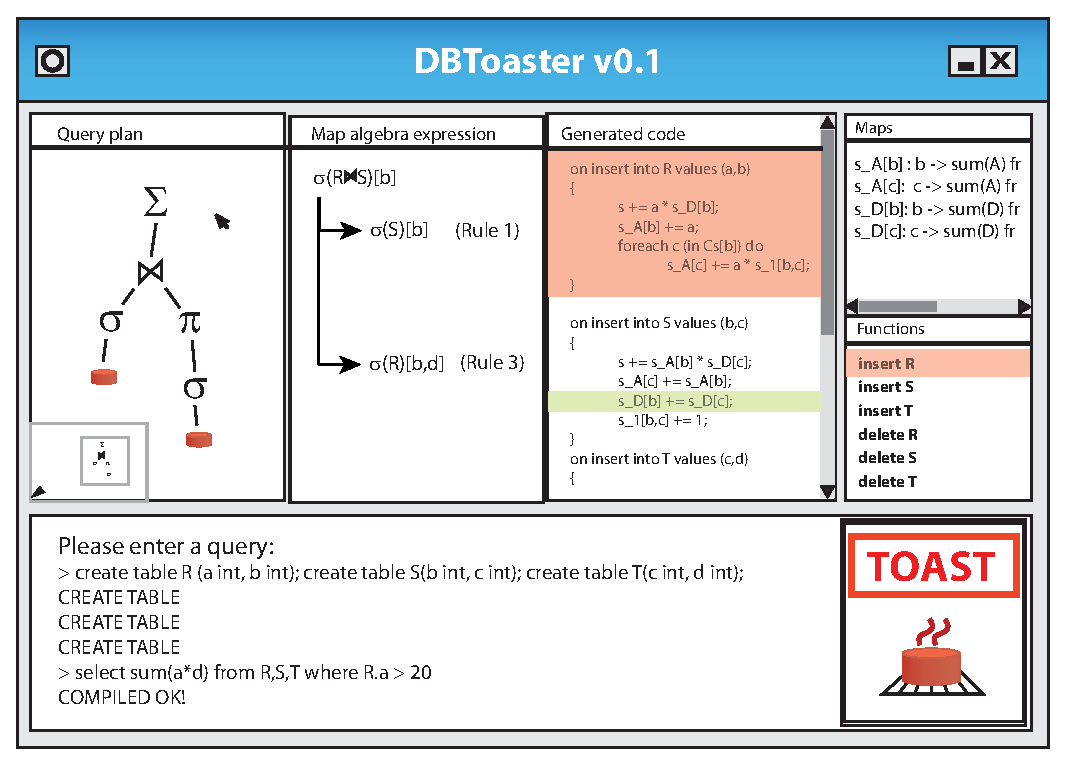
\includegraphics[scale=0.47]{figures/gui1}
\end{center}
\caption{\compiler\ compilation process visualization, displaying map algebra
transformations, generated code, and internal views that must be maintained.}
\label{fig:compilegui}
\end{figure}

The first of our two visualization tools (Figure~\ref{fig:compilegui} above) aids
in conveying the compilation process to demo attendees. We will invite attendees
to input their own queries, or use one of the canned queries from our
applications, and first visually display a standard relational query plan. Our
visualizer will then display the transformation process in a step-by-step fashion
by applying rewrite rules in our map algebra, allowing us to explain the contents
of the maps built from the query. In the next phase of the demonstration, we will
briefly describe the code generation process given these maps, and how we can
derive code to maintain these maps using only the bottom layer of the query as an
example, where map maintenance proves to be simple. At this point query
compilation is complete, and we implement a pair of simple browser windows
listing both the maps and the tuple functions generated to allow access to
arbitrary steps in the compilation process, to aid in discussions with attendees.
\comment{
Depending on the
demonstration progress, we may additionally include an example of a
JIT-compilation of the example query to demonstrate the potential for a limited
degree of adaptivity during query execution.
}

\subsection{\compiler\ vs. DBMS* Bakeoff}
The theme in this part of the demonstration is to show \compiler's
competitiveness with a variety of database tools, by performing a DBMS bakeoff.
Our experiments\footnote{under submission.} have demonstrated \compiler\ is able
to significantly outperform PostgreSQL and a naive approach to query compilation
for both the automated trading application and data loading application, as well
as the Stanford STREAM~\cite{motwani-cidr:03} engine for Linear Road. In
addition to these three comparison points we plan to compare to
HSQLDB~\cite{hsqldb-url}, an existing pure Java main-memory database. The second
visualization tool displays the performance achieved by the compiled query
executors generated in the above part of the demonstration. The metrics of
interest here are the throughput \compiler\ achieves, its memory usage for
maintaining its maps as part of tuple function processing, the binary size, and
finally the compile time including both the C++ generation and the subsequent
compilation to a native binary. To provide for a more entertaining audience
experience, we will run an audience challenge to find queries both yielding the
greatest performance over the other database engines in the bakeoff, as well as
queries that illustrate the poorest performance. Attendees will be provided with
two laptops at the demonstration booth to experiment with queries, and we will
display a leaderboard of the running results to spur on competition.


%\footnotesize{
\bibliographystyle{abbrv}
\bibliography{ref}
%}

\end{document}
